% Designed Companion Part IV figure
% Intended for \input{...} beside the matching canonical problem.
\begin{figure}[ht]
\centering
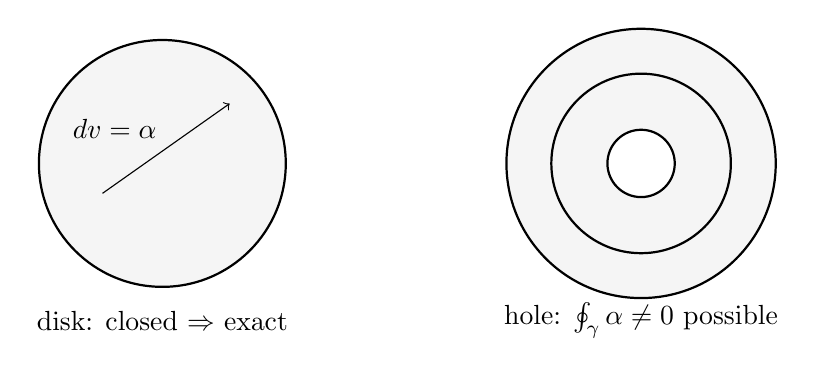
\begin{tikzpicture}[scale=0.95]
  \begin{scope}[xshift=-3.2cm]
    \fill[gray!8] (0,0) circle (1.65);
    \draw[thick] (0,0) circle (1.65);
    \draw[->] (-0.8,-0.4)--(0.9,0.8) node[midway,above left] {$dv=\alpha$};
    \node at (0,-2.1) {disk: closed $\Rightarrow$ exact};
  \end{scope}
  \begin{scope}[xshift=3.2cm]
    \fill[gray!8] (0,0) circle (1.8);
    \fill[white] (0,0) circle (0.45);
    \draw[thick] (0,0) circle (1.8);
    \draw[thick] (0,0) circle (0.45);
    \draw[->,thick] (0,0) circle (1.2);
    \node at (0,-2.1) {hole: $\oint_\gamma\alpha\ne0$ possible};
  \end{scope}
\end{tikzpicture}
\caption{For harmonic $u$, the conjugate differential $\alpha=-u_y\,dx+u_x\,dy$ is closed. On a disk it is exact and produces a harmonic conjugate; on a multiply connected domain a nonzero loop integral can obstruct a global conjugate.}
\label{fig:cp-iv-0126-harmonic-conjugate-local-global}
\end{figure}
